\documentclass[tikz]{standalone}
\begin{document}
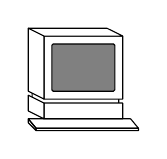
\begin{tikzpicture}[rounded corners=.1pt]
    \draw (-.15,-.1) rectangle (.95,.5);
    \draw[fill=white] (0,0) rectangle (1,.8);
    \draw[fill=white] (0,0) -- (-.2,.1) -- (-.2,.9) -- (.8,.9) -- (1,.8) -- (0,.8) --
    cycle;
    \draw (0,.8) -- (-.2,.9);
    \draw[fill=white] (0,-.05) -- (1,-.05) -- (1,-.25) -- (0,-.25) -- cycle;
    \draw[fill=white] (0,-.05) -- (0,-.25) -- (-.2,-.15) -- (-.2,.05) -- cycle;
    \draw[rounded corners=.5pt,fill=gray] (.1,.1) rectangle  (.9,.7);
    \draw (-.2,-.25) -- (1.1,-.25) -- (1.2,-.37) -- (-.1,-.37) -- cycle;
    \draw (-.2,-.25) -- (-.2,-.3) -- (-.1,-.4) -- (-.1,-.37) -- cycle;
    \draw (-.1,-.4) rectangle (1.2,-.37);
\end{tikzpicture}
\end{document}